\chapter{Tests}

In diesem Kapitel werden zu den drei Design Patterns die jeweiligen Testfälle erläutert.

\section{Singleton}

Um sicherzustellen, dass die Singleton-Klasse richtig implementiert worden ist, müssen neben dem Behandeln der Compiler-Fehler und Warnungen folgende Testfälle manuell überprüft werden: 

\begin{description}
  \item[1.]
  Als allererstes muss überprüft werden, ob der Standard-Konstruktor der Singleton-Klasse aufrufbar ist. Sollte dies der Fall sein, scheitert der Test, denn der Konstruktor sollte von außerhalb nicht aufrufbar, d.h. private sein.
  \begin{itemize}
  \item{Durchführung:}
  In Rhapsody wurde versucht, eine Instanz der Singleton-Klasse zu erzeugen.
  \item{Ergebnis:}
  Der Build in Rhapsody ist fehlgeschlagen, da der Konstruktor private ist. Der
  Test ist erfolgreich.
  \end{itemize}
  \begin{figure}[!htbp]
	\centering
	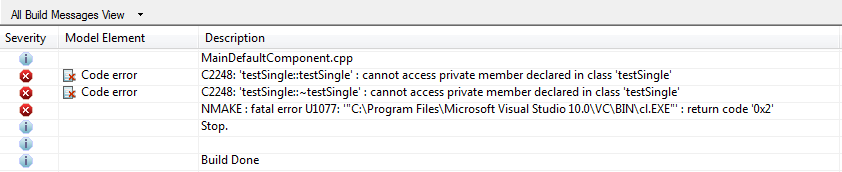
\includegraphics[width=0.99\textwidth]{content/pictures/tests/singleton/error1}
	\label{pic:bild}
	\caption{Fehler beim Zugriff auf privaten Konstruktor}
\end{figure}
  \item[2.]
  Weiterhin muss überprüft werden, ob man von einem bestehenden Singleton-Objekt eine Kopie erzeugen kann. Ist dies möglich, scheitert dieser Test, denn ein Singleton-Objekt darf nicht kopiert werden. Der Copy-Konstruktor muss auch private sein.
  \begin{itemize}
  	\item{Durchführung:}
  	In Rhapsody wurde versucht, eine Instanz der Singleton-Klasse einer Variablen
  	zuzuordnen.
  	\item{Ergebnis:}
  	Der Build in Rhapsody ist fehlgeschlagen, da der Kopierkonstruktor private
  	ist.
  	Der Test ist erfolgreich.
  \end{itemize}
  
 \begin{figure}[!htbp]
	\centering
	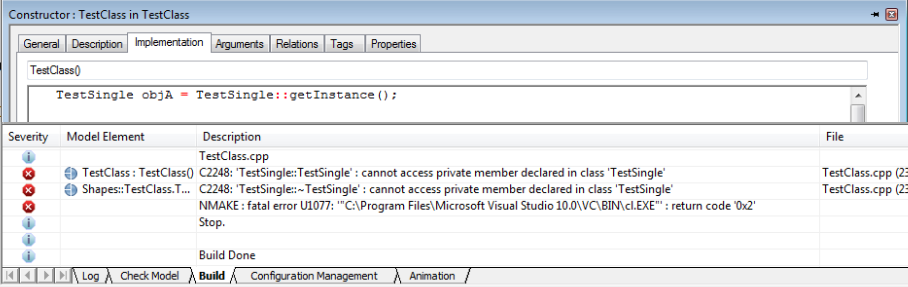
\includegraphics[width=0.99\textwidth]{content/pictures/tests/singleton/KopierError1}
	\label{pic:bild}
	\caption{Fehler bei Kopier-Konstruktor}
\end{figure}
  
  \item[3.]
  Ein weiterer Test ist, dass geprüft werden muss, ob es möglich ist, ein Singleton-Objekt zur Laufzeit zu zerstören. Das Singelton-Objekt wird erst am Ende der Programmlaufzeit freigegeben. Kann das Objekt schon vorher zerstört werden, schlägt der Test fehl. Der Destruktor muss auch als private deklariert sein.
  \begin{itemize}
  	\item{Durchführung:}
  	In Rhapsody wurde versucht, ein Singleton-Object zur Laufzeit zu zerstören.
  	\item{Ergebnis:}
  	Der Build in Rhapsody ist fehlgeschlagen, da der Destruktor pirvate ist. Der
  	Test ist erfolgreich.
  \end{itemize}
  \begin{figure}[!htbp]
	\centering
	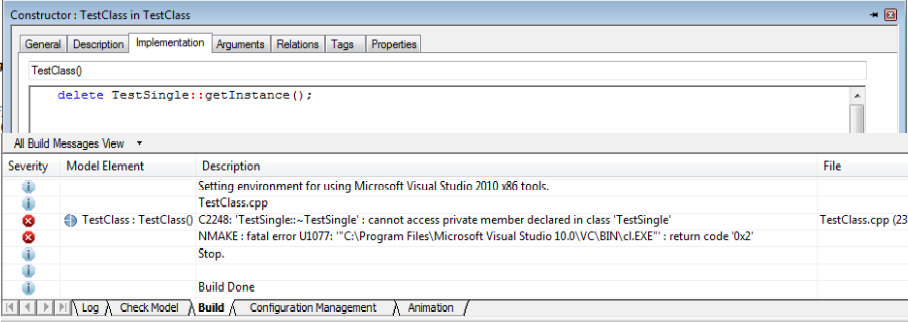
\includegraphics[width=0.99\textwidth]{content/pictures/tests/singleton/deleteError1}
	\label{pic:bild}
	\caption{Fehler beim Löschen des Objekts}
\end{figure}

  \item[4.]
  Möchte man von außerhalb ein Objekt der Singleton-Klasse implementieren, muss dies über die einzige öffentliche Methode der Singleton-Klasse "GetInstance()" passieren. Hierbei wird ein neues Objekt angelegt, sofern noch keins vorhanden war, ansonsten wird einfach das "alte" Objekt zurückgegeben.
  \begin{itemize}
  	\item{Durchführung:}
  	In Rhapsody wird zweimal eine Singleton-Instanz angefordert.
  	\item{Ergebnis:}
  	Der Build in Rhapsody ist erfolgreich. Beim ersten Anfordern einer
  	Singleton-Insatnz wurde eine neue Instanz erstellt, beim zweiten Aufruf wurde
  	die bestehende Instanz zurückgegeben.
  	Der Test ist erfolgreich.
  \end{itemize}
  
  \item[5.]
  Hat der Benutzer selbst eine GetInstance-Methode implementiert, muss Rhapsody bei der Erzeugung des Projektes einen Fehler ausgeben und die Erzeugung abbrechen.
  \begin{itemize}
  \item{Durchführung:}
  In Rhapsody wurde versucht, einer Klasse, die bereits eine getInstance()
  Methode beinhaltet, den Stereotyp <<Singleton>> zuzuordnen.
  \item{Ergebnis:}
  Der Build in Rhapsody ist nicht fehlgeschlagen. Der Test ist nicht
  erfolgreich.
  \end{itemize}
  \begin{figure}[!htbp]
	\centering
	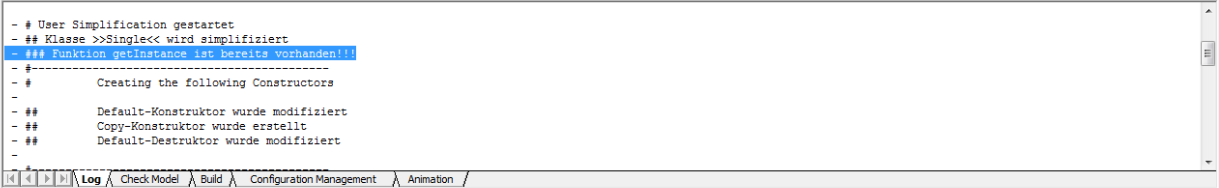
\includegraphics[width=0.999\textwidth]{content/pictures/tests/singleton/getinstanceerror1}
	\label{pic:bild}
	\caption{Fehler bei vorhandener getInstance-Methode}
\end{figure}

  \item[6.]
  Nachdem das Singelton-Objekt mithilfe der getInstance()-Methode erzeugt wurde, liefert diese Methode stets die gleiche Instanz der Singleton-Klasse zurück. 
  \begin{itemize}
  	\item{Durchführung:}
  	In Rhapsody wurden mehrere Singleton-Instanzen angefordert.
  	\item{Ergebnis:}
  	Der Build in Rhapsody war erfolgreich. Bei jeder angeforderten Instanz
  	wurde der gleiche Pointer zurückgegeben. Der Test ist erfolgreich.
  \end{itemize} 
  \begin{figure}[!htbp]
	\centering
	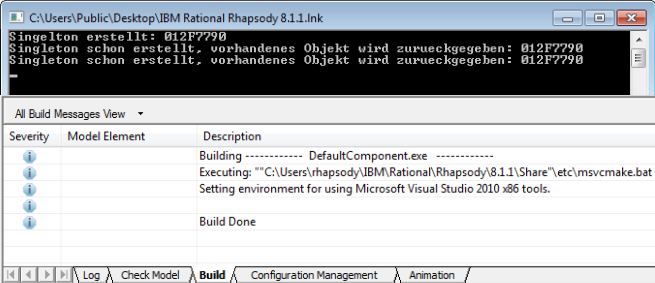
\includegraphics[width=0.9\textwidth]{content/pictures/tests/singleton/HappyDay1}
	\label{pic:bild}
	\caption{Happy-Day bei der Simplification von Singleton}
\end{figure}
 
\end{description}

\section{Observer}

Um sicherzustellen, dass das Observer Pattern richtig implementiert worden ist, müssen neben dem Behandeln der Compiler-Fehler und Warnungen folgende Testfälle manuell überprüft werden: 

\begin{description}

	\item[1.]
	Hat der Benutzer bereits eine Klasse namens Observer oder Subject oder deren Methoden implementiert, muss Rhapsody die Simplification mit Fehlermeldung abbrechen.
	
	\item[2.]
	Wenn der Benutzer nur einen der Observer/Subject Stereotypen zugewiesen hat, muss Rhapsody das Programm übersetzen, aber eine entsprechende Warnung ausgeben.
	
	\item[3.]
	Eine bestimmte Anzahl Observer werden am Subject registriert, danach wird die Anzahl der registrierten Observer überprüft. Diese Anzahl muss mit der eingegebenen Anzahl übereinstimmen. \\
	Dadurch wird sichergestellt, dass alle Observer registriert wurden.

	\item[4.]
	Mehrere Observer werden am Subject registriert, danach wird eine bestimmte Anzahl wieder gelöscht. Die Anzahl der registrierten Observer muss den Anfangs registrierten minus den gelöschten Observern entsprechen.
	
	\item[5.]
	Es wird versucht, einen Observer zu löschen, ohne dass vorher ein Observer am Subject registriert wurde.Hierbei darf kein Fehler passieren.
	 
	\item[6.]
	An einem Subject werden mehrere Observer registriert. Diese beinhalten eine einfache Implementierung, die einen Text auf der Konsole ausgeben. Dadurch kann leicht überprüft werden, ob alle Observer durch die notify()-Funktion benachrichtigt und die jeweiligen Update()-Funktion aufgerufen wurde.
	
	\item[7.]
	Es wird ein Modell angelegt, bei dem die Methoden register/unregister und update schon im subject vorhanden sind. Beim Versuch der Simplification muss Rhapsody hier einen Fehler ausgeben und den Vorgang abbrechen.
	
	\item[8.]
	Es wird ein Modell angelegt, bei dem die Klassen Object und Subject manuell hinzugefügt wurden. Beim Versuch der Simplification muss Rhapsody hier einen Fehler ausgeben und den Vorgang abbrechen.
	
	\item[9.]
	Es wird zweimal hintereinander eine Simplification auf ein gültiges Modell angewandt. Beim zweiten Duchgang soll Rhapsody einen Text ausgeben, der darüber informiert, dass die Klassen Subject und Observer bereits simplifiziert wurden, und bei dem aktuellen Vorgang ignoriert werden.

\end{description}


\section{Guarded Call}

Auch für das letzte Pattern sind einige Tests nötig. Viele verschiedene Faktoren
haben Einfluss auf die Simplification.
\begin{description}

	\item[1.]
	Bei den ersten Tests wird wie bei den anderen Design Pattern überprüft ob die Namenskonvention eingehalten werden. Im Falle des Guarded Call wird getestet ob der Name für das Mutex-Attribut bereits vergeben ist. Wenn dies der Fall ist, soll eine Meldung gezeigt werden, damit der Benutzer daraufhin den Namen anpassen kann.
	
	\item[2.]
	Wenn der vorgesehene Name des Mutex-Attributs noch frei ist muss überprüft werden ob der Datentyp der Variable auch dem gewünschten Typ \textit{OMOSMutex*} (plattformunabhängige Mutex von Rhapsody, siehe Beschreibung von Guarded Call) entspricht. Ebenso muss getestet werden ob das Attribut korrekt initialisiert wird.
	
	\item[3.]
	Die Funktionsnamen müssen geprüft werden. An den Benutzerfunktionen wird das Wort "Guarded" angehängt. Wenn eine Funktion schon diese Endung hat, darf die Funktion nicht weiter bearbeitet werden und es folgt wieder eine Meldung an den Benutzer.
	
	\item[4.]
	Es muss getestet werden ob die Funktionen, die vom Benutzer erstellt wurden, korrekt umbenannt und auf private gesetzt wurden. Ebenso muss überprüft werden ob in der ursprünglichen Funktion die Wrapper-Funktion richtig erstellt wird.
	
	\item[5.]
	Es muss geprüft werden, ob der Funktionsaufruf in der Wrapper-Funktion korrekt von einem try-catch Block eingeschlossen wird. Dabei muss getestet werden ob die in der aufgerufenen Funktion geworfene Exception abgefangen, die Mutex entsperrt und anschließend die abgefangene Exception erneut geworfen wird.
	
	\item[6.]
	Da immer alle Funktionen des Objekts gesperrt werden muss überprüft werden, ob weitere Threads vor dem Ausführen einer geschützten Funktion auch tatsächlich gesperrt werden sollte bereits ein Thread sich in einer geschützten Funktion befinden.
	
	\item[7.]
	Ebenso sollte überprüft werden ob es sich beim Mutexobjekt um eine rekursive Mutex handelt. Dabei muss getestet werden, ob ein Thread sich selbst ausschließt wenn innerhalb einer geschützten Funktion eine Wrapper-Funktion aufgerufen wird.
	
	\item[8.]
	Es muss getestet werden ob der Datentyp des Rückgabewerts bei der Wrapper-Funktion und der geschützten Funktion gleich sind und ob beide Funktionen den gleichen Wert zurückgeben.
	
	
\end{description}
